\documentclass[10pt,a4paper,twocolumn]{article}

\usepackage[T1]{fontenc}
\usepackage[utf8]{inputenc}

\usepackage[english]{babel}
\usepackage{natbib}
\usepackage{url}

\usepackage{graphicx, grffile}
\graphicspath{{./assets_ipr/}}

\usepackage{booktabs}

\title{
  Intellectual Property, Technological Innovation,
  \\ and Academic Research: Lecture Notes
}
\author{Nazarov Ivan}
\date{April 2020}


\begin{document}

\maketitle

\section{IP Overview} % (fold)
\label{sec:intellectual_property_overview}

\begin{quote}
  Intellectual property is that class of intangible assets on which legal rights have
  been conferred by a sovereign state whereby the recipients of those rights possess
  the authority to exclude others from using, making, selling, distributing, importing,
  copying or otherwise exploiting the associated assets without permission.
\end{quote}

Trademark -- distinguishing signs of the origin of a product or service.

Trade secret -- information, that is not generally known, which provides commercial
competitive advantage, and which is actively kept secret and protected.
\begin{itemize}
  \item source code, process, chemical formulae
  \item user or client databases, pending patents
\end{itemize}
Intangible asset, must be defined articulated and notified as sensitive and protected
information.

Patent -- a property title on technical idea, teaching or invention. Conveys exclusive
rights granted by a state within the jurisdiction of its IP law to an ``inventor'' for
a limited term, in exchange for full public disclosure (`quid pro quo'). Regarded as
personal property.

Design rights -- protect the appearance of products.

Copyright -- intellectual rights in works of science, literature and art, which exist
in some objective form.
\begin{itemize}
  \item computer code are considered an object of copyright and protected as literary
  works
  \item works of authorship fixed in any tangible medium of expression
\end{itemize}
Copyright protection term: lifetime plus seventy years. Purchase is not copyright ownership
transfer.

Copyright does not extend to ideas, functions, concepts, theories, schemes, principles,
methods, rules, programming languages etc. Patents protect ideas as such, copyright
relates only to the expression of thereof.

Patents may protect the underlying technical ideas, functionality and useful features of
the software. Copyright may protect the literal expression of the code.

Berne Convention of 1986 declared that computer software/ programme (object code and
the source code) and the compilation of the data should be protected under the Copyright
Acts. Programmes are nothing more than scientific discoveries, laws of nature or mathematical
formulae. Representations in form of instructions, of a mathematical formula or a
relationship which could be applied in a number of ways, sometimes also referred to as
algorithms.

\subsection{Patents in Different Countries} % (fold)
\label{sub:patents_in_different_countries}

Patents confer a right to the patentee to exclude another from making, selling or using
the invention without a license, for 20 years from the date a patent is applied for. A
patent is owned by an inventor until it has been assigned to another party. A license
typically gives a licensee a right to use or sub-license the invention. Licenses are
valuable for commercialization because it as a market entry barrier for non-licensed
competitors.

A patentable inventions a result of intellectual activity which meets the requirements:
\begin{itemize}
  \item (RUS, GER) must involve an \textit{inventive step} and be industrially applicable
  \item (US) new, useful process, machine, manufacture or composition of matter, or any
  new improvement thereof
  \item (CHN) must be novel, creative and of practical use, solve a technical problem
  \item (AUS, NZ) manner of manufacture, or applicable to improvement or control of
  manufacture.
\end{itemize}
Essentially a new, useful and non-obvious invention is patentable.


Subject matter of patents or inventions should involve a technical teaching, i.e. an
instruction addressed to a skilled practitioner as to how to solve a particular technical
problem using particular technical means. Must not be an abstract creation (mathematical
theorem of formula), but one that produces a given practical result, such as new device,
or a new method of producing an existing product. Commercial success might be used to
demonstrate usefulness and ``non-obviousness''.

``Non-obviousness'' means the invention is regarded by other practitioners in the field
as ingenious. And that which would not have been created in the course of ordinary
activities of a practitioner, i.e. requiring an inventive step. Non-obviousness to an
expert with ordinary skill in the art, an ordinary practitioner, possessing of common
general knowledge in the art at the relevant time.

Novelty means not anticipated by ``prior art'' anywhere in the world. The \emph{state of
the art} is everything made available to the public by means of a written or oral description,
by use, or in any other way, before the date of filing of the patent application.
%
There are differences in each legislature regarding the \textit{priority} dates: first to
invent, first to file, first inventor to file. In some countries there is 12-month grace
period for printed publications or other forms of public disclosure (in scientific journal
or thesis), before in is considered ``prior art''.

Disclosure means that an invention must be disclosed with sufficiently complete information,
so that a person, \textit{skilled in the art} cloud implement it without \textit{undue}
experimentation or effort. By being disclosed, the invention is reduced to practice.

Conceived an invention is much more involved than imagined it: needs a proof of concept.

In RU, EU, and China patents are subject to morality and public safety/order clauses.

% subsection patents_in_different_countries (end)

\subsection{``per se'' or ``as such''} % (fold)
\label{sub:per_se_or_as_such}

``Program for a computer ... \textbf{as such}'' means binary executable. ``per se'' refers
to something on its own rather than in connection with other things, i.e. scripting languages
(interpreted) in a Virtual Machine; code and ideas, methods, and algorithms, but not their
particular realisation itself (binary, which spins in production, or higher level).

``computer program per se'' not a particular expression in high level language, object or
binary, but a general composition of method and algorithms, business logic, and interface.
Business methods, even if implemented using a computer and a computer program, are nonetheless
considered as non-patentable. Other matter is a new or an improved method of doing business,
or a new or an improved algorithm, or a new or an improved mathematical method.

% subsection per_se_or_as_such (end)

\subsection{``Four Factor Test''} % (fold)
\label{sub:_four_factor_test_}

The plaintiff must demonstrate
\begin{itemize}
  \item suffered irreparable injury
  \item remedies available, e.g. monetary damages, are deemed inadequate compensation
  \item considering the balance of hardships, a remedy in equity is warranted
  \item and that the public interest would not be disserved by a permanent injunction
\end{itemize}

% subsection _four_factor_test_ (end)

\subsection{Basic Intellectual Property Transfer Process} % (fold)
\label{sub:basic_intellectual_property_transfer_process}

The key figures in this process are:
\begin{itemize}
  \item[A] creator, original source of IP (employee, researcher)
  \item[B] primary organization, owner of IP (employer, university)
  \item[C] secondary organization, intermediate user of IP (licensee, startup)
  \item[D] customer, end user of IP (private citizen)
\end{itemize}
The process itself involves the following flows:
\begin{itemize}
  \item A $\longrightarrow$ B assignment of ownership
  \item B $\longrightarrow$ C licensing the right to use the IP
  \item C $\longrightarrow$ D selling product or service embodying IP rights
\end{itemize}
The patenting process:
\begin{itemize}
  \item[$\longrightarrow$] Inventing
  \item[$\longrightarrow$] Preparation for a patent application
  \item[$\longrightarrow$] Preparation and filing a patent application
  \item[$\longrightarrow$] ``Prosecuting'' a patent application
  \item[$\longrightarrow$] Maintaining patent registration
\end{itemize}
``Appropriating value from a patent'' can
\begin{itemize}
  \item[$\longrightarrow$] enforcing patent rights directly or by litigation
  \item[$\longrightarrow$] re-inventing
\end{itemize}
\begin{figure}
  \centering
  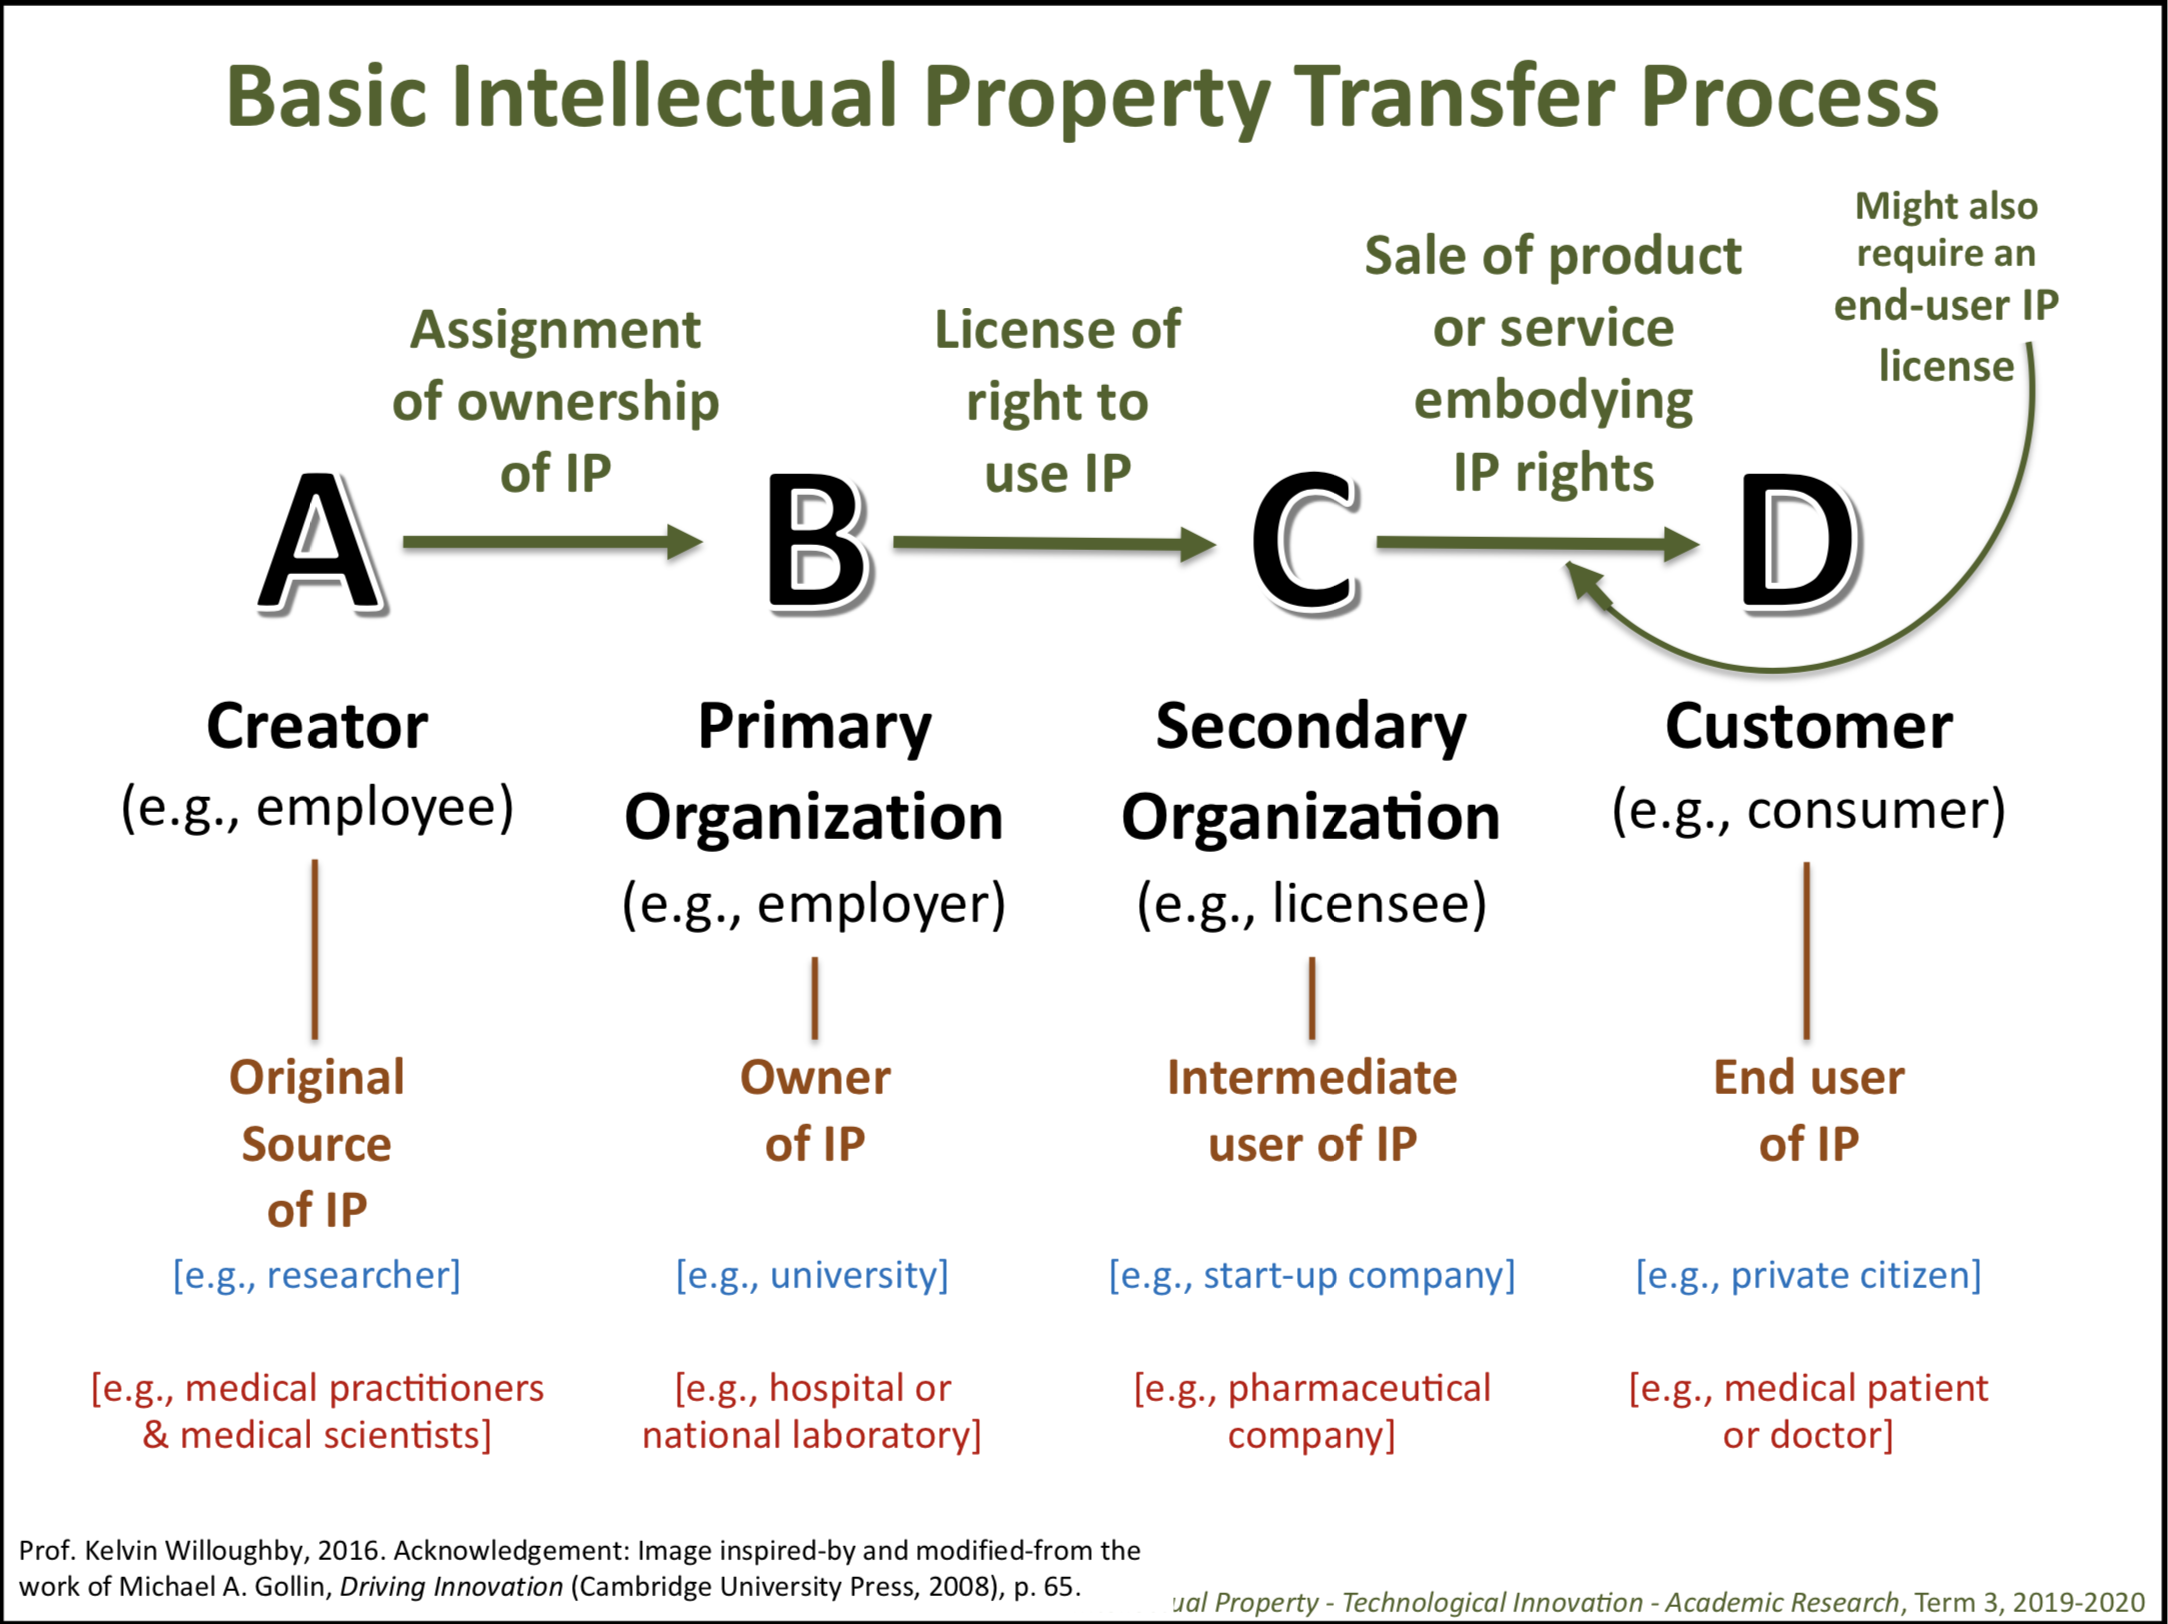
\includegraphics[width=\columnwidth]{basic_ip_transfer.png}
\end{figure}

% subsection basic_intellectual_property_transfer_process (end)

% section intellectual_property_overview (end)

\section{Copyright and DRM} % (fold)
\label{sec:copyright_and_drm}

Intellectual rights in works of science, literature, and art are considered subject to
copyright rights.

Filing for copyright is easy: just create and make (fix) a manifestation in a tangible
medium of expression. By default copyright confers an exclusive right to the creator.
This right is automatic right, which arises by the sheer act of creating a work.

Moral rights: the holder has the right to object to any distortion, mutilation, or other
modification of, or other derogatory action in relation to the said works, which would
be prejudicial to their honour or reputation.

Copyright is the right to expression of the content, and not the rights to a physical copy,
which the end user possesses. Copyright is inapplicable to technical ideas, theories, means,
solutions -- only to the expression of ideas. For example, the literal expression of the
code, the underlying technical idea, functionality of features.

Both source code and object code are copyrighted (binary executable?).

It is illegal under Russian law and foreign laws to make copies of computer software
without the permission of the owner of the copyright of that software. However, there
are exceptions: the owner of a copy can copy, without copyright holders' consent,
\begin{itemize}
  \item to decompile for legitimate purposes
  \item to modify the programme to enable it to work on the technical means
  \item to correct critical faults, errors
  \item as a back up, for study or research
\end{itemize}

What is fair use? It is the reproduction of copyrighted material for purposes such as
criticism, comment, news reporting, teaching, scholarship or research. Important elements
are:
\begin{itemize}
  \item purpose and character of use, the amount and substantiality of the portion used
  \item effect of the use in the potential market for or value of the copyrighted work
\end{itemize}

In Australia, no renting, no unauthorized use of copies (selling and otherwise). Reproduction
and adaptation is acceptable for the normal technical use of software, which it was designed
for: study, security testing, backup, make interoperable with products, correcting errors.

In software, as everywhere, licensing does not mean transferring ownership.

\begin{figure}
  \centering
  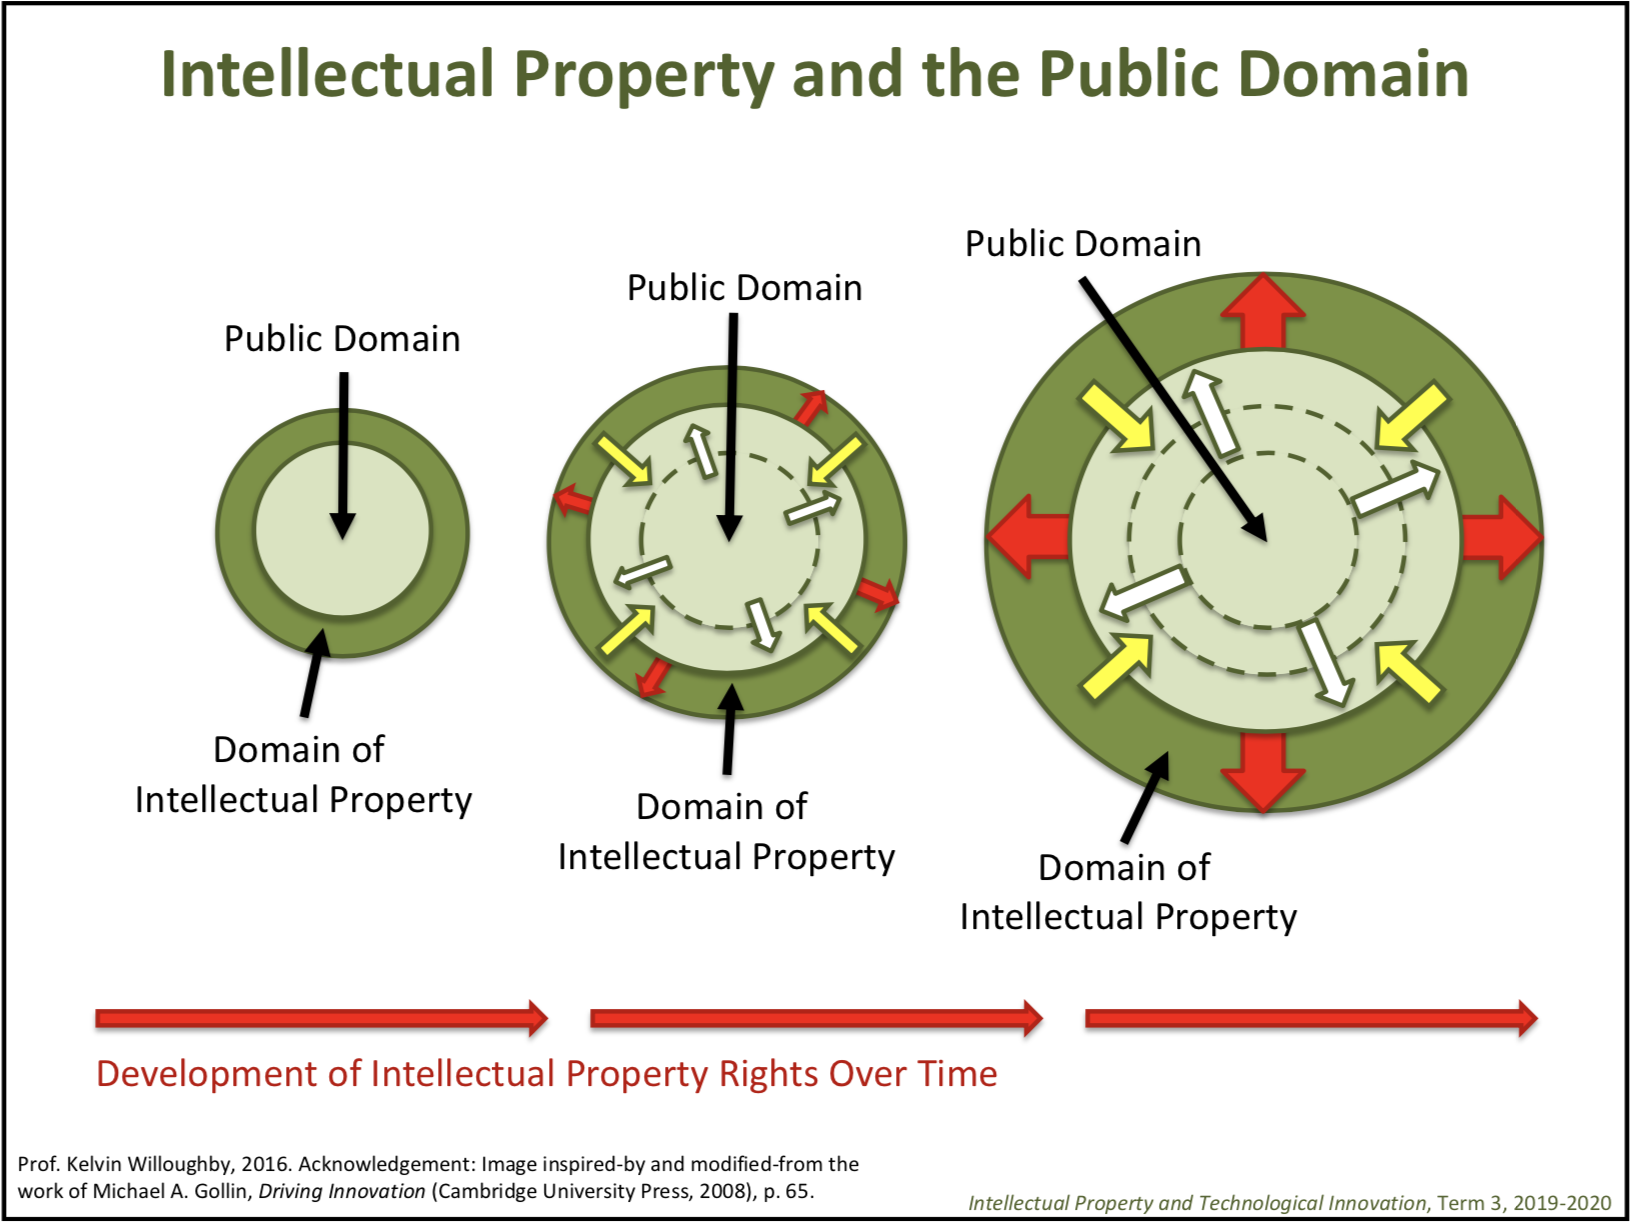
\includegraphics[width=\columnwidth]{ip_and_pb.png}
\end{figure}
\begin{figure}
  \centering
  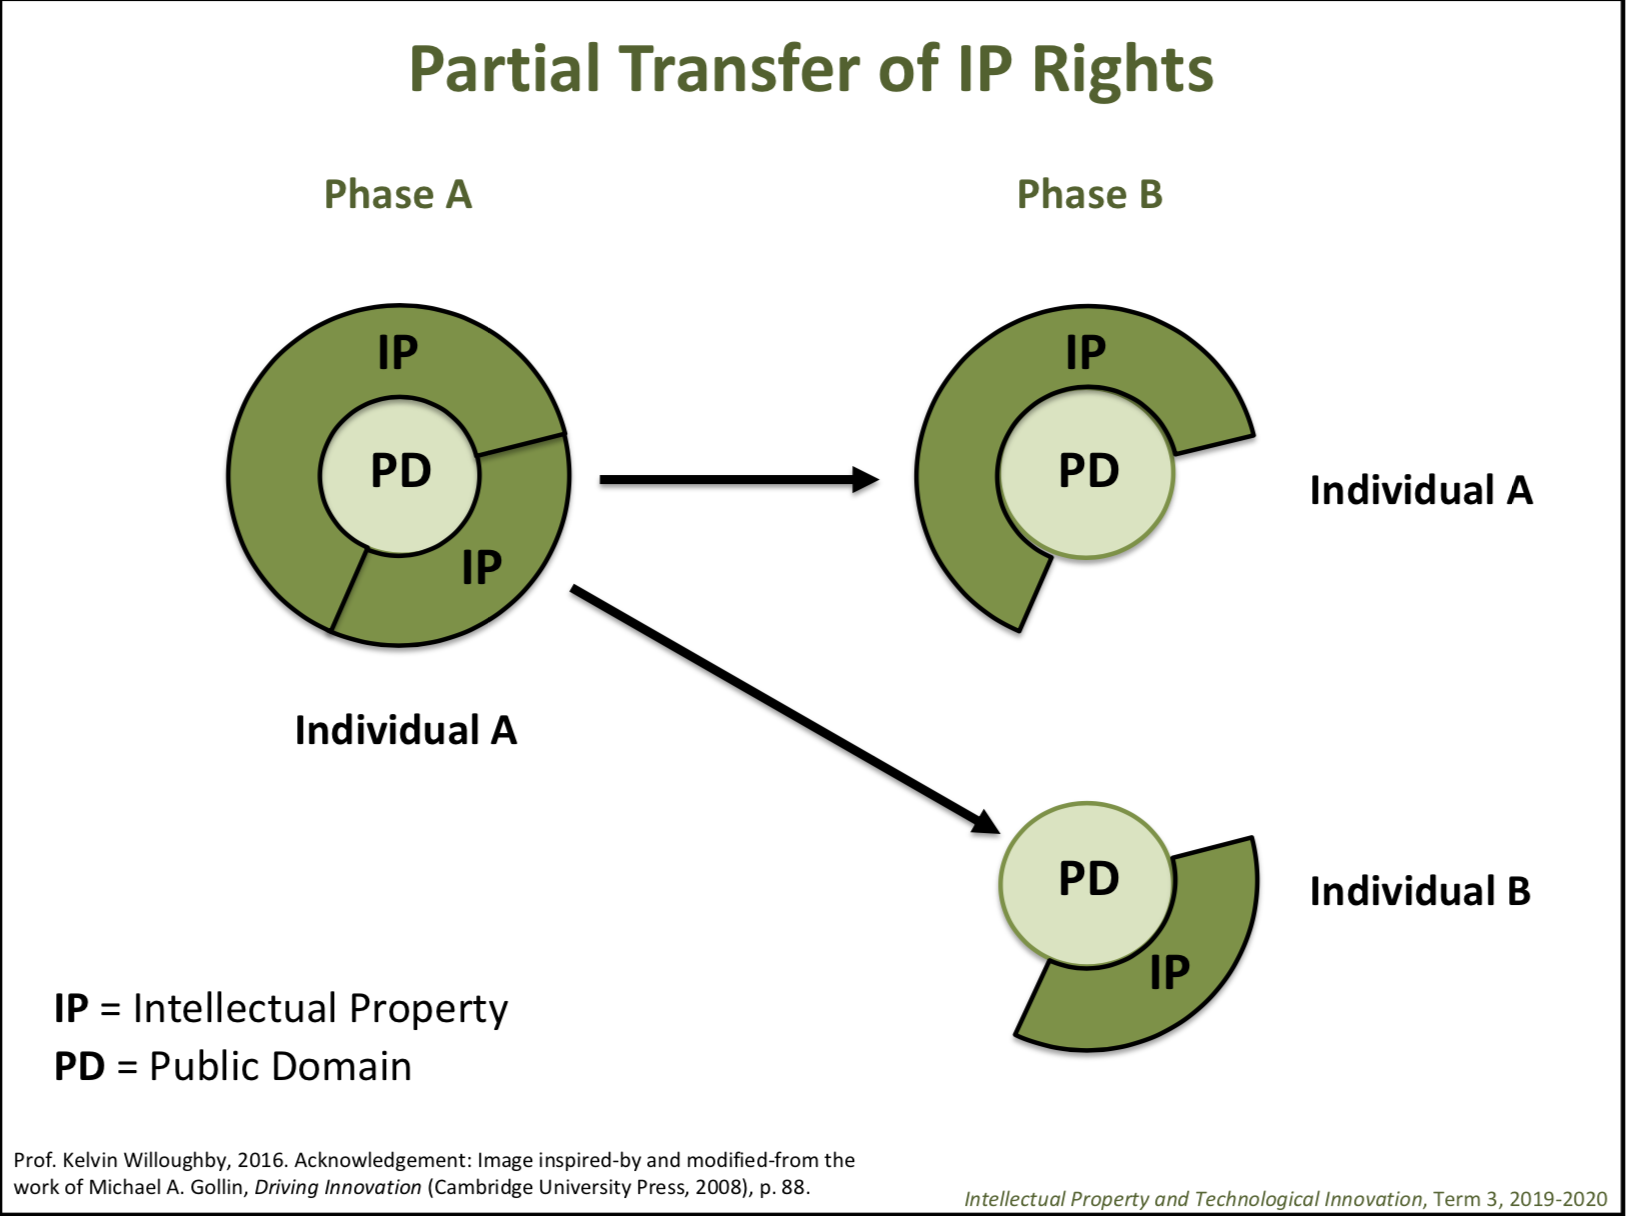
\includegraphics[width=\columnwidth]{ip_partial.png}
\end{figure}
\begin{figure}
  \centering
  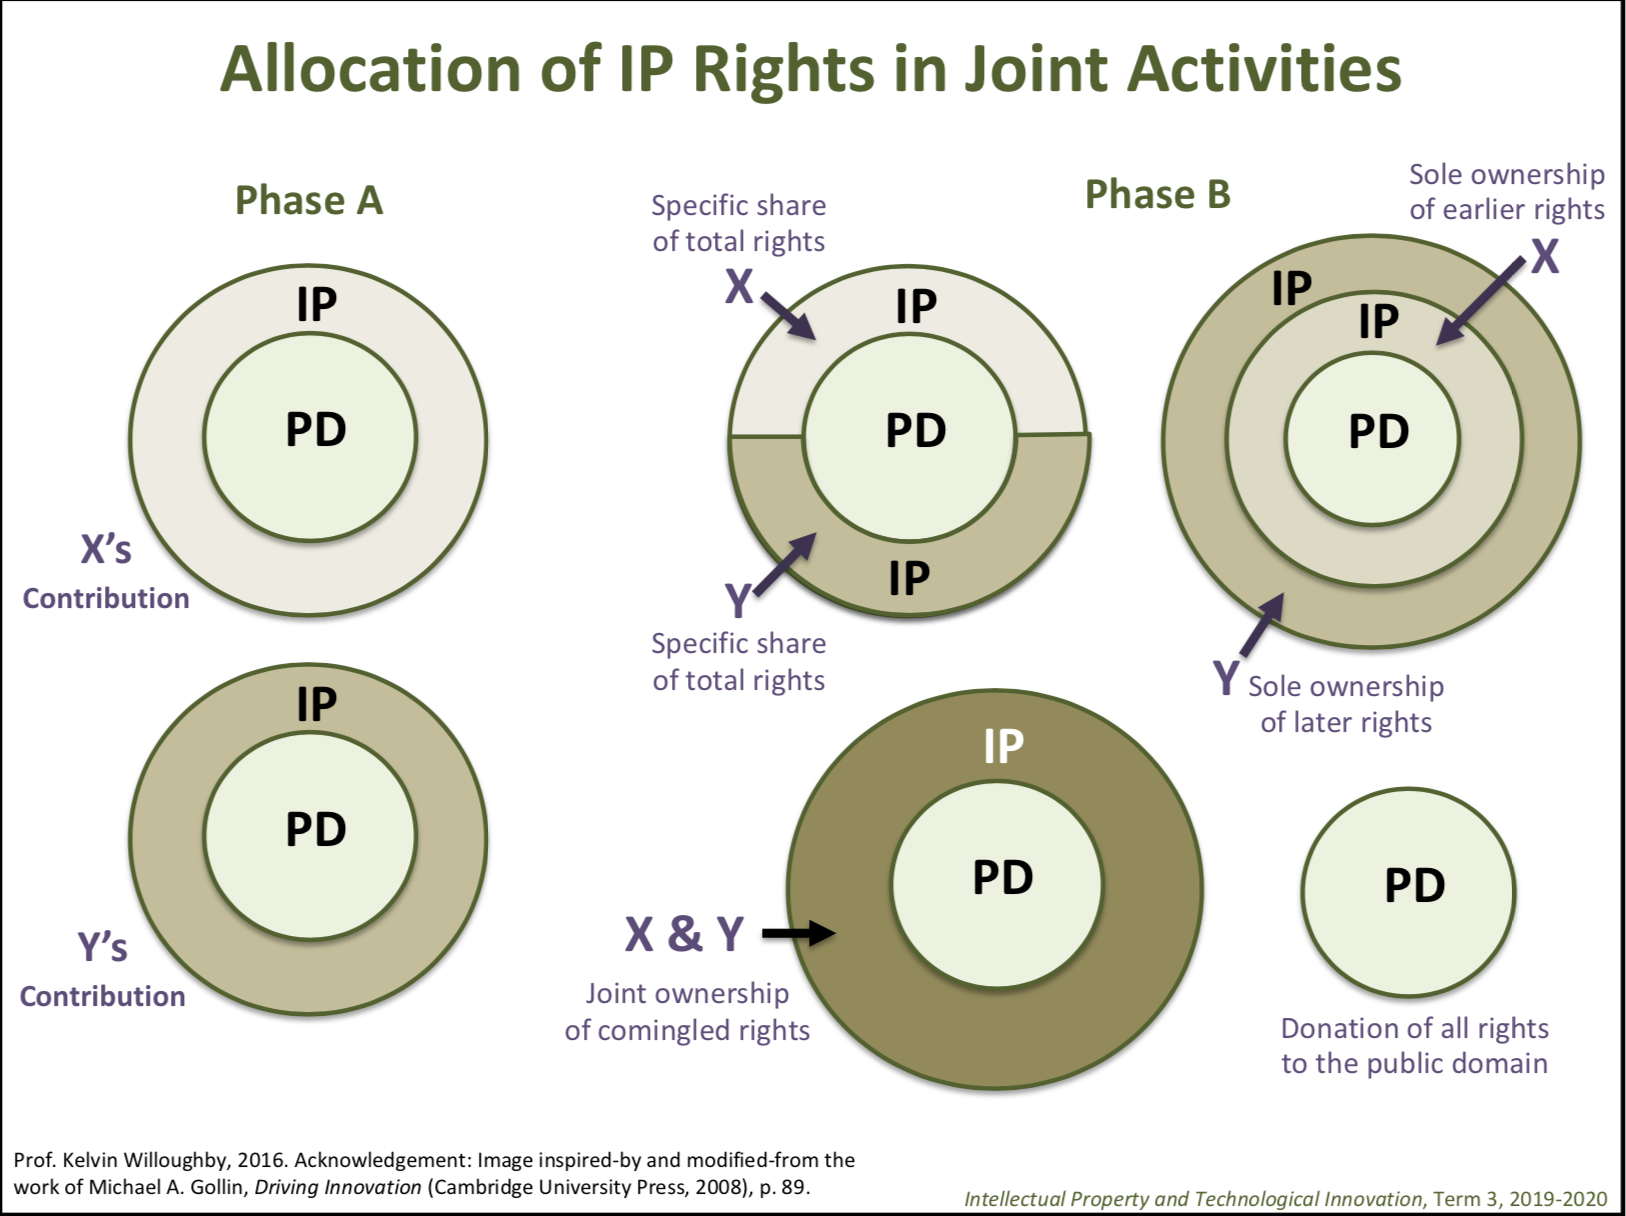
\includegraphics[width=\columnwidth]{ip_allocation.png}
\end{figure}

% section copyright_and_drm (end)

\section{Trademarks} % (fold)
\label{sec:trademarks}

Trademarks are distinguishing elements to identify the source or origin of goods or services.
Has signalling purposes: quality assurance, recognition, goodwill, sign of a genuine product.

Trademark must be a sign capable of individualising goods and services of legal entities
or individual entrepreneurs. A valid sign includes a word, name, symbol, device, slogan,
product shape, or other designation. The holder of a trademark is granted an exclusive right
by registering a TM to use it, or authorize other to use it. Trademark must be visual, and
be capable of being graphically represented. The essential feature of a trademark s that
it must be distinctive in itself, and be able to identify and distinguish, or indicate the
source. Expires when a trademark becomes a generic name, falls into disuse by its owner,
changes the designated product, service or industry.

Infringement: identical of sufficiently similar goods so as to likely cause confusion.

The spectrum for trademarks essential features:
(robust, distinctive) $\leftarrow$ fanciful, arbitrary, suggestive, descriptive,
generic $\rightarrow$ (desirable).

% section trademarks (end)

\section{Trade secrets} % (fold)
\label{sec:trade_secrets}

Trade secrets and confidential information. This is secretive, actively protected, and
indicated as such information, method, process, that is of significant importance to
the owning business, has actual or potential economic value, or gives a competitive edge
(code, recipe, technique, database, pending patents, patterns).
\begin{itemize}
  \item not generally known
  \item provides commercial advantage
  \item actively kept as a secret
  \item articulated in a document
\end{itemize}
Ceases to be a trade secret if becomes public information, hence must be maintained
as a secret.
\begin{itemize}
  \item a non-disclosure agreement, confidentiality agreement, non-compete agreement
  \item security access
\end{itemize}
Trade secrets are not protected by intellectual property laws, so
\begin{itemize}
  \item reverse engineering
  \item independent discovery or invention
\end{itemize}
is not illegal. Although may conflict with the license agreement or copyright restrictions.

Trade secrets become public domain, if leaked, stolen, patented, or published. Patents
enable design rights and trademarks. There are no access restrictions on the intellectual
property committed to public domain.

% section trade_secrets (end)

\section{Design patents} % (fold)
\label{sec:design_patents}

Engineering designs are technical functionality, back end or model. Design patents relate
to aesthetics of industrial and engineering designs (like UI and UX):
\begin{itemize}
  \item artistic, outward appearance
  \item aesthetics, ergonomics, shape
  \item apparent configuration, ornament, colours
\end{itemize}
Design is inseparable from the article, to which it is applied and cannot exist alone,
like an interface. To be patentable it must be new and original, i.e. not generally
known before the priority date. Strike a balance between functionality and aesthetics.

% section design_patents (end)

\section{Licensing} % (fold)
\label{sec:licensing}

Licensing intellectual property is a direct source of income from the IP assets. License
is a contract, a legally binding promise between consenting parties, a licensor, and a
licensee, that states: Licensor, a holder of the exclusive rights to an IP grants, or
undertakes a commitment to grant, the licensee, the other party, the right to use the
intellectual property within limits and subject to terms and only if expressly indicated.
\begin{quote}
  Licensing intellectual property involves the licensor granting the right to use the
  intellectual property to the licensee. Typically, this was a long-term business relationship
  between the licensor and the licensee. The latter pays for the right to use the IP, by
  way of either lump-sum of instalment payments. A licensor has the flexibility to structure
  the license arrangement and any obligations alongside the process by which the licensee
  pays for the License. Further restrictions could be placed so that IP could only be used
  for a particular class of products or geographical location.
\end{quote}

Agreement is a contract, if it is legally valid, i.e. written, officially registered. Presumes
\begin{itemize}
  \item offer and acceptance with genuine consent
  \item intention for legally binding relations, having legal capacity
  \item assumes an exchange of value
\end{itemize}

% section licensing (end)

\section{Ownership} % (fold)
\label{sec:ownership}

University retains the ownership of service results of intellectual on the part of employees
and students, except copyright in scientific publications and student dissertations.
\begin{figure}
  \centering
  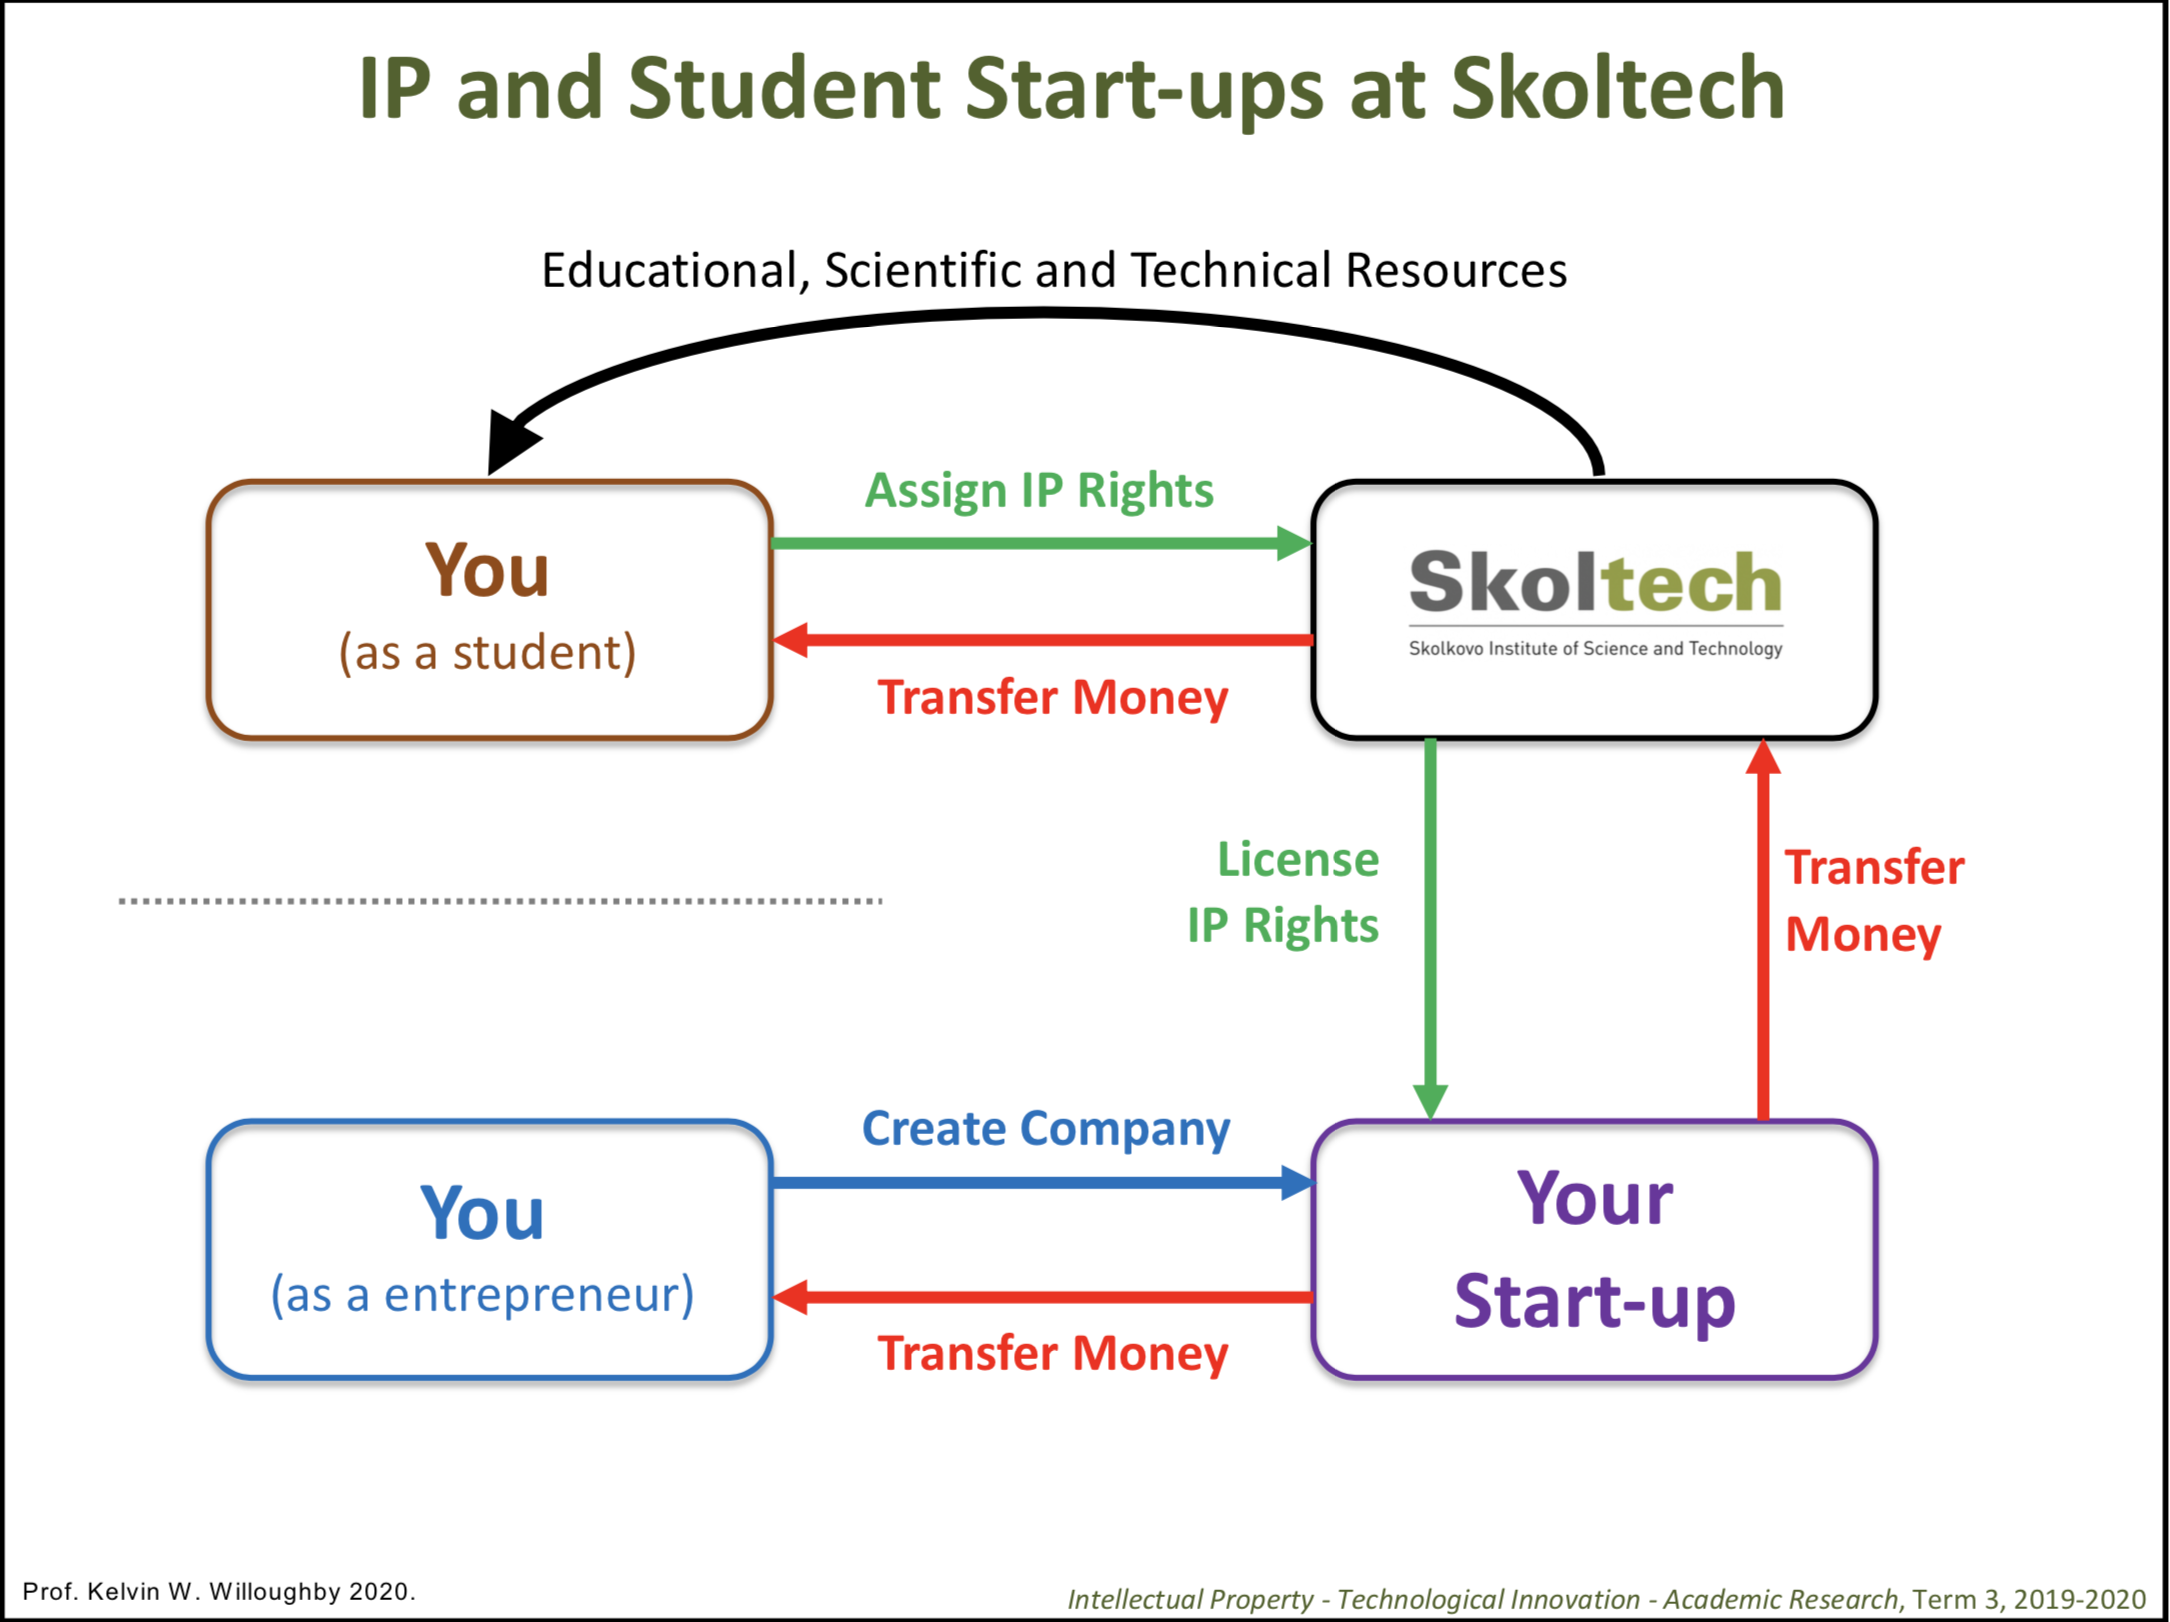
\includegraphics[width=\columnwidth]{student_and_uni.png}
\end{figure}

% section ownership (end)

\section{Intellectual Property and Industrial Standards} % (fold)
\label{sec:intellectual_property_and_industrial_standards}

Industry standards are established when innovative technology enters a phase of consolidation
and incremental change. Standards secure the technology and help achieve economies of scale
and integration.

Standards are elements of technical systems
\begin{itemize}
  \item refer to and define the architecture of technical systems
  \item ``hardened'' officially codified technical knowledge
  \item shared technical knowledge
\end{itemize}
Modularity, linkage, interoperability; community adoption,; ``locking in'' -- maintaining
de facto control, and building institutionalized support. And keep IP rights to the pivotal
elements of the standard.

Standards work when they are implemented and complied with. They regulate recommended
practices too. They are published documents that establish specifications and procedures
designed to ensure reliability.
\begin{itemize}
  \item consistent protocols, that can be universally understood and adopted
  \item helps interoperability and compatibility, simplifies product development,
  facilitates comparison
  \item provides means of verification of credibility
\end{itemize}
ISO standards avoid patented items, but if it is necessary to make reference to patented
items, then licenses to those patented items must be made available worldwide on Fair,
Reasonable and Non-Discriminatory terms.

No standards and too many standards is equally bad.

% section intellectual_property_and_industrial_standards (end)

% \bibliographystyle{abbrvnat}

% \bibliography{references}

\end{document}
